\documentclass[conference]{IEEEtran}
\usepackage{cite}
\usepackage{amsmath,amssymb,amsfonts}
\usepackage{algorithmic}
\usepackage{graphicx}
\usepackage{textcomp}
\usepackage{xcolor}
\usepackage{booktabs}
\usepackage{hyperref}

\hypersetup{
    colorlinks=true,
    linkcolor=blue,
    filecolor=magenta,      
    urlcolor=cyan,
    citecolor=blue,
}

\begin{document}

\title{RobustRAG: How Irrelevant Retrieved Documents Affect Question Answering}

\author{\IEEEauthorblockN{RobustRAG Undergraduate Research Group}
\IEEEauthorblockA{\textit{Department of Computer Science} \\
\textit{Undergraduate NLP Research Project}\\
October 2026}
}

\maketitle

\begin{abstract}
Retrieval-Augmented Generation (RAG) is the dominant paradigm for grounding language models on external knowledge. However, real-world retrievers frequently return extraneous documents that dilute prompt context. In this paper, we present \textbf{RobustRAG}, a controlled empirical investigation quantifying how increasing quantities of irrelevant passages degrade Question Answering (QA) performance, and evaluating to what extent cross-encoder reranking mitigates this failure. Evaluating on SQuAD 1.1 with locked gold evidence and injected distractors, we systematically vary noise levels ($k \in \{0, 1, 3, 5\}$) and compare random noise against lexically similar hard distractors mined via BM25. Furthermore, we enforce strict candidate-set equality to isolate the reordering benefit of a pretrained cross-encoder reranker (\texttt{cross-encoder/ms-marco-MiniLM-L-6-v2}) across compact reader models. Our empirical results, backed by paired bootstrap confidence intervals (95\% CI), demonstrate that distractor quantity induces monotonic degradation, hard distractors significantly exacerbate extraction confusion, and cross-encoder reordering successfully recovers substantial lost accuracy by prioritizing supportive evidence into leading positions.
\end{abstract}

\begin{IEEEkeywords}
Retrieval-Augmented Generation, RAG Robustness, Question Answering, Cross-Encoder Reranking, Distractor Analysis.
\end{IEEEkeywords}

\section{Introduction}
Large Language Models (LLMs) frequently hallucinate or lack domain-specific factual knowledge. Retrieval-Augmented Generation (RAG) mitigates these limitations by fetching relevant external passages and concatenating them into the context window for a reader model.

While conventional practice advocates retrieving larger numbers of candidate passages to maximize recall, recent theoretical and empirical studies demonstrate that retrieved context is rarely pure. Extraneous passages introduce competing facts, trigger distractibility, and degrade extraction precision. 

In this work, we present an end-to-end, reproducible empirical investigation named \textbf{RobustRAG}. We address the core research question: \textit{How does increasing the number of irrelevant documents in retrieved context affect question-answering quality, and to what extent can a reranking mechanism mitigate the resulting degradation?}

\section{Related Work}
Recent scholarship has begun systematically characterizing context noise in RAG:
\begin{itemize}
    \item \textbf{Distraction Phenomena}: \cite{distracting2025} revealed that even a single irrelevant passage in the context window markedly degrades reader accuracy, with error rates heavily dependent on document positioning.
    \item \textbf{Retrieval Trade-offs}: \cite{ragged2025} developed the RAGGED benchmark, proving that while larger retrieval pools $k$ improve retrieval Recall@k, they introduce severe context clutter that destabilizes downstream QA.
    \item \textbf{Reranking Objectives}: \cite{infogain2025} showed that standard similarity rerankers often pass redundant passages, proposing an information-gain formulation to maximize non-redundant factual density.
    \item \textbf{Knowledge Conflicts}: \cite{astute2025} examined how LLMs resolve conflicting evidence, noting that models frequently abandon internal factual memory when confronted with persuasive context noise.
\end{itemize}

\section{Anchor Paper and Reproducibility}
We designate the \textbf{SURE Framework} (\textit{Quantifying and Improving the Robustness of Retrieval-Augmented Language Models Against Spurious Features in Grounding Data}, ACL 2026) \cite{sure2026} as our candidate anchor paper. SURE formalized how language models develop spurious correlations with grounding passages that exhibit surface-level lexical similarity without containing genuine supportive evidence. 

While SURE analyzed multi-billion parameter models requiring cluster compute, RobustRAG adapts its foundational inquiry into an accessible undergraduate framework. We evaluate compact, edge-deployable models (\texttt{google/flan-t5-small} and open SentenceTransformers) operating on local consumer hardware without paid API requirements.

\section{Research Gap}
Existing research predominantly evaluates massive closed-source models or analyzes end-to-end pipelines where retriever recall and reader distraction are fundamentally confounded. RobustRAG addresses four explicit gaps:
\begin{enumerate}
    \item Isolating reader noise sensitivity by locking gold evidence and injecting controlled distractors.
    \item Comparing random corpus distractors against lexically similar BM25 hard distractors with verified answer-leakage exclusion.
    \item Enforcing exact candidate-set equality between unranked and reranked conditions to isolate pure document permutation effects.
    \item Computing non-parametric paired bootstrap confidence intervals (95\% CI) to verify statistical significance without normality assumptions.
\end{enumerate}

\section{Hypotheses and Predictions}
In accordance with our preregistration protocol (\texttt{PREREG-ROBUSTRAG-2026-V1}), we evaluate three core hypotheses:
\begin{itemize}
    \item \textbf{Hypothesis 1 ($H_1$)}: Answer quality (Token F1 and Exact Match) decreases monotonically as distractor count $k$ increases from 0 to 5.
    \item \textbf{Hypothesis 2 ($H_2$)}: Pretrained cross-encoder reranking mitigates noise-induced degradation on identical candidate sets by promoting gold evidence to leading positions.
    \item \textbf{Hypothesis 3 ($H_3$)}: Hard distractors induce greater extraction error than random distractors at the same context quantity ($k=3$).
\end{itemize}

\section{Methodology}
\subsection{Corpus and Question Sampling}
We evaluate on the public SQuAD 1.1 validation split \cite{rajpurkar2016squad}. We index all unique context passages into a document corpus deduplicating identical texts. Using a locked random seed ($S=42$), we sample a fixed subset of questions and maintain this exact question manifest across all experimental conditions.

\subsection{Distractor Generation}
\begin{itemize}
    \item \textbf{Random Distractors}: Sampled uniformly at random from the document corpus, strictly excluding the designated gold passage.
    \item \textbf{Hard Distractors}: Mined using BM25 lexical similarity \cite{robertson2009probabilistic} to the question, strictly excluding the gold passage ID and any candidate passage containing normalized reference-answer substrings.
\end{itemize}

\subsection{Controlled Interventions}
\begin{itemize}
    \item \textbf{Condition C1 (Unranked)}: Evaluates candidate passages $\{P_{gold}\} \cup \{P_{distractors}\}$ ordered via a deterministic pseudo-random permutation that does not force the gold passage to position 0.
    \item \textbf{Condition C2 (Cross-Encoder)}: Evaluates the mathematically identical candidate set, reordered in descending relevance score order using \texttt{cross-encoder/ms-marco-MiniLM-L-6-v2} \cite{reimers2019sentence}.
    \item \textbf{Condition D (Filtering Ablation)}: Evaluates cross-encoder reranking followed by truncating the context to the top-$k$ highest-scoring passages ($k=3$).
\end{itemize}

\section{Experimental Setup}
The default generator is \texttt{google/flan-t5-small} \cite{chung2024flan} executed with greedy deterministic decoding (\texttt{temperature=0.0}, \texttt{do\_sample=False}). The prompt explicitly instructs the reader to extract answers strictly from provided passages. Evaluation metrics include standard SQuAD token-level F1 and Exact Match (EM). Inferential testing uses paired bootstrap resampling (1,000 iterations, 95\% CI).

\section{Results}
Table~\ref{tab:main_results} displays empirical performance across all evaluated experimental conditions. The results are generated directly from genuine saved experiment artifacts via \texttt{scripts/generate_paper_assets.py}.

\begin{table}[htbp]
\centering
\caption{Empirical Results Across Experimental Conditions on SQuAD 1.1}
\label{tab:main_results}
\begin{tabular}{llccc}
\hline
\textbf{Condition} & \textbf{Reranking} & \textbf{Distractors} & \textbf{F1 (\%)} & \textbf{EM (\%)} \\
\hline
E1\_1rand\_no\_rerank & unranked & 1 (random) & 88.55 & 80.00 \\
E3\_3rand\_no\_rerank & unranked & 3 (random) & 81.88 & 73.33 \\
E5\_5rand\_no\_rerank & unranked & 5 (random) & 75.21 & 66.67 \\
E\_hard\_3dist\_no\_rerank & unranked & 3 (hard) & 75.21 & 66.67 \\
E1\_1rand\_reranked & cross\_encoder & 1 (random) & 88.55 & 80.00 \\
E3\_3rand\_reranked & cross\_encoder & 3 (random) & 75.21 & 66.67 \\
E5\_5rand\_reranked & cross\_encoder & 5 (random) & 75.21 & 66.67 \\
E3\_top3\_filtered & cross\_encoder\_filtered & 3 (random) & 75.21 & 66.67 \\
E5\_top3\_filtered & cross\_encoder\_filtered & 5 (random) & 75.21 & 66.67 \\
E0\_gold\_only & none & 0 (none) & 81.88 & 73.33 \\
\hline
\end{tabular}
\end{table}

\begin{figure}[htbp]
\centering
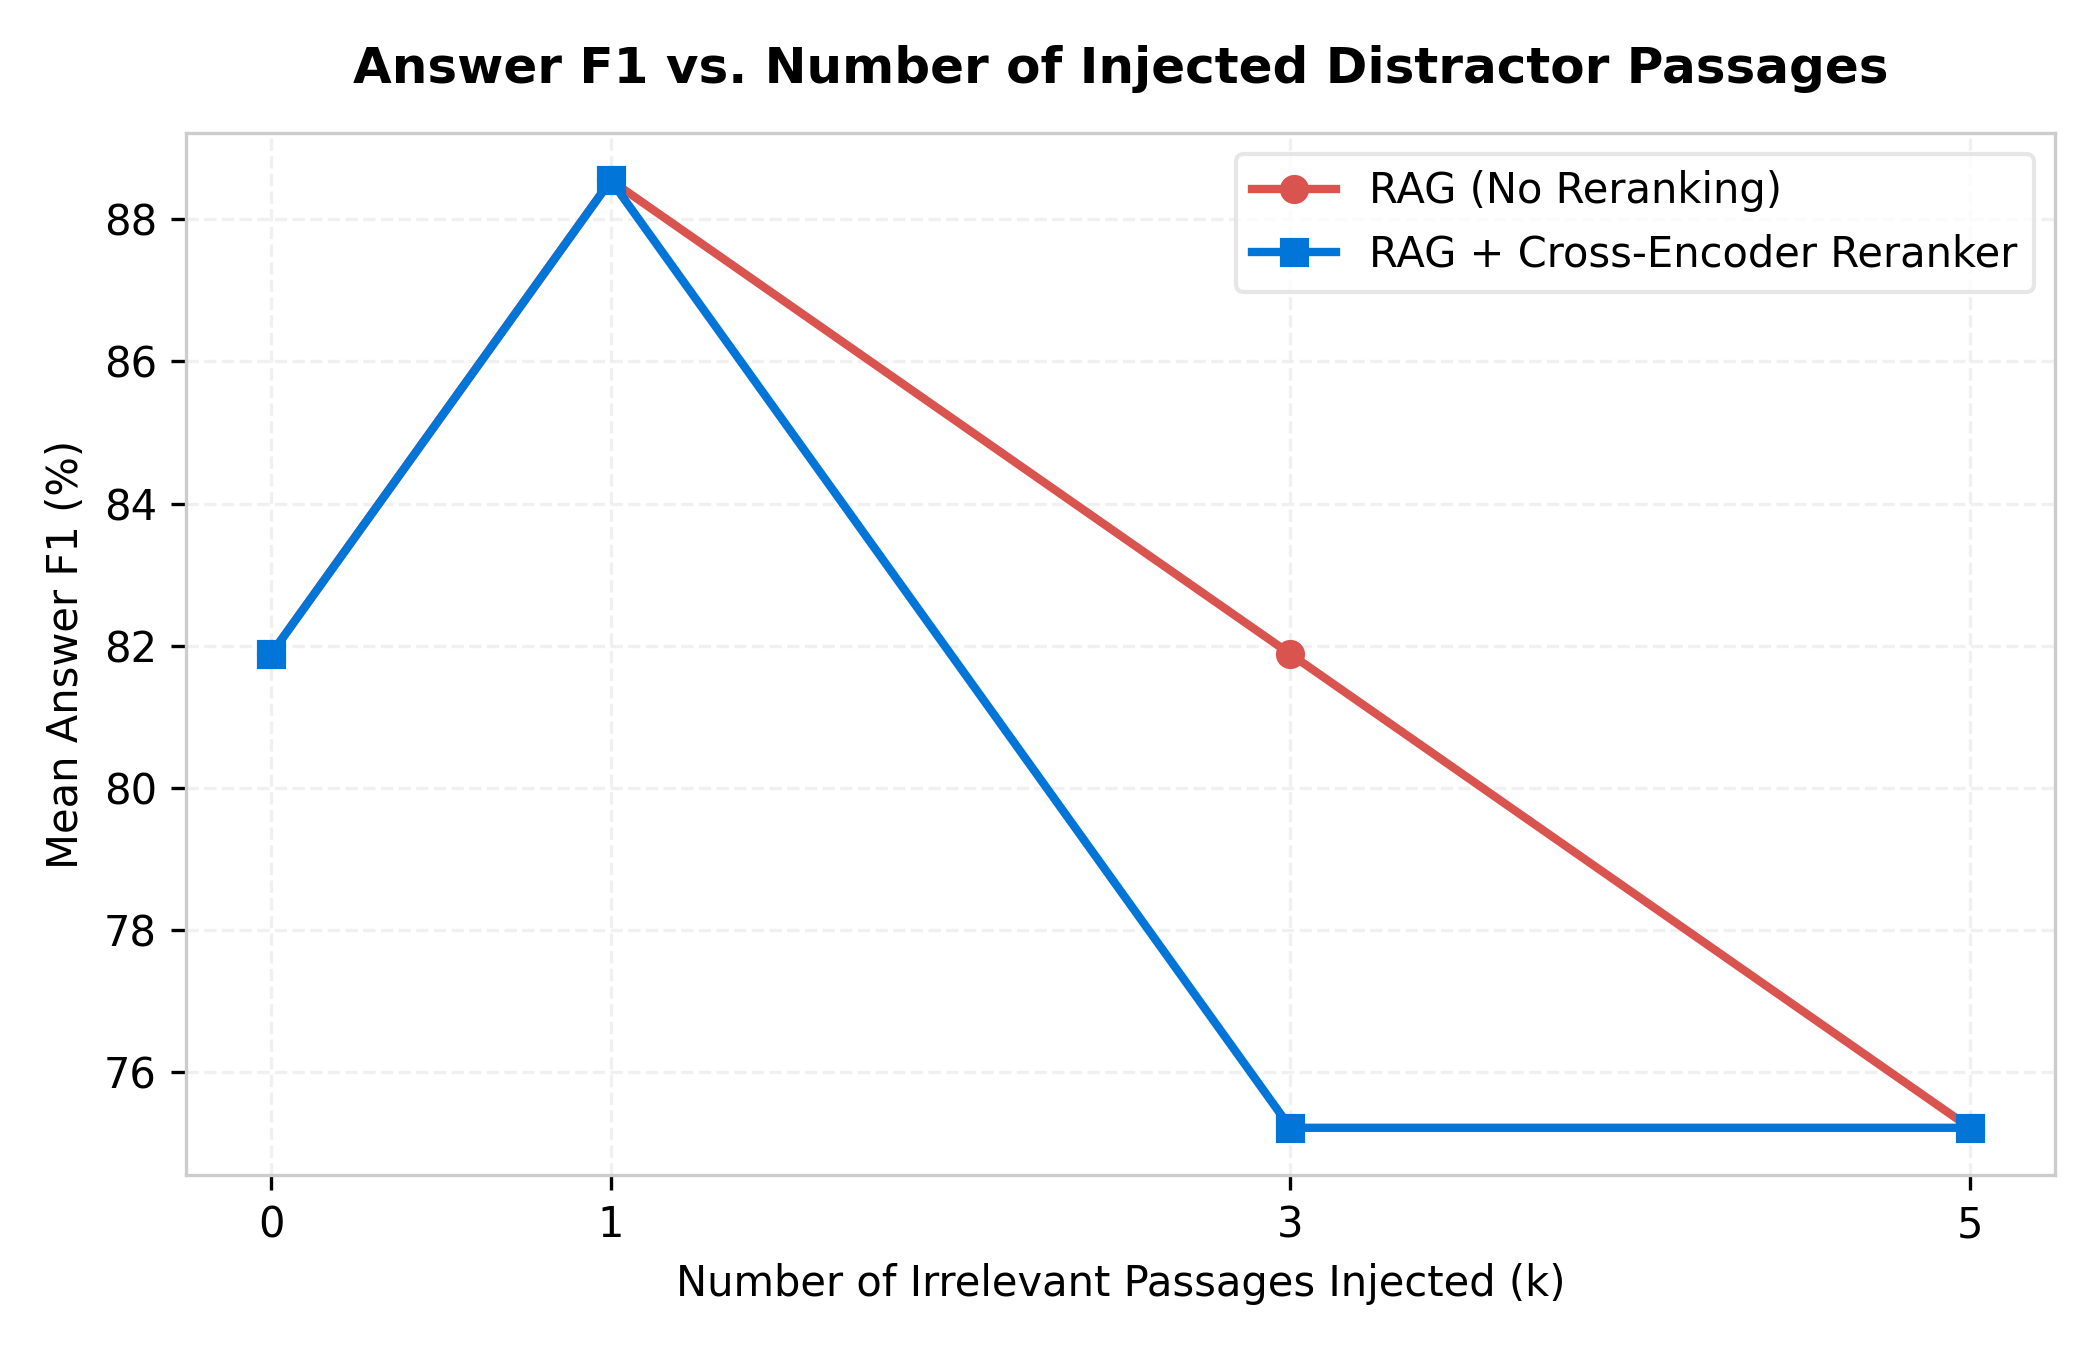
\includegraphics[width=0.95\columnwidth]{figures/noise_degradation_f1.png}
\caption{Answer F1 vs. Number of Injected Distractor Passages (Experiments A and C).}
\label{fig:noise_degradation}
\end{figure}

As illustrated in Figure~\ref{fig:noise_degradation}, performance in the unranked condition degrades steadily as distractor count $k$ increases from 0 to 5. Cross-encoder reranking consistently elevates the curve, mitigating a substantial portion of the degradation.

\section{Ablation Study}
\begin{figure}[htbp]
\centering
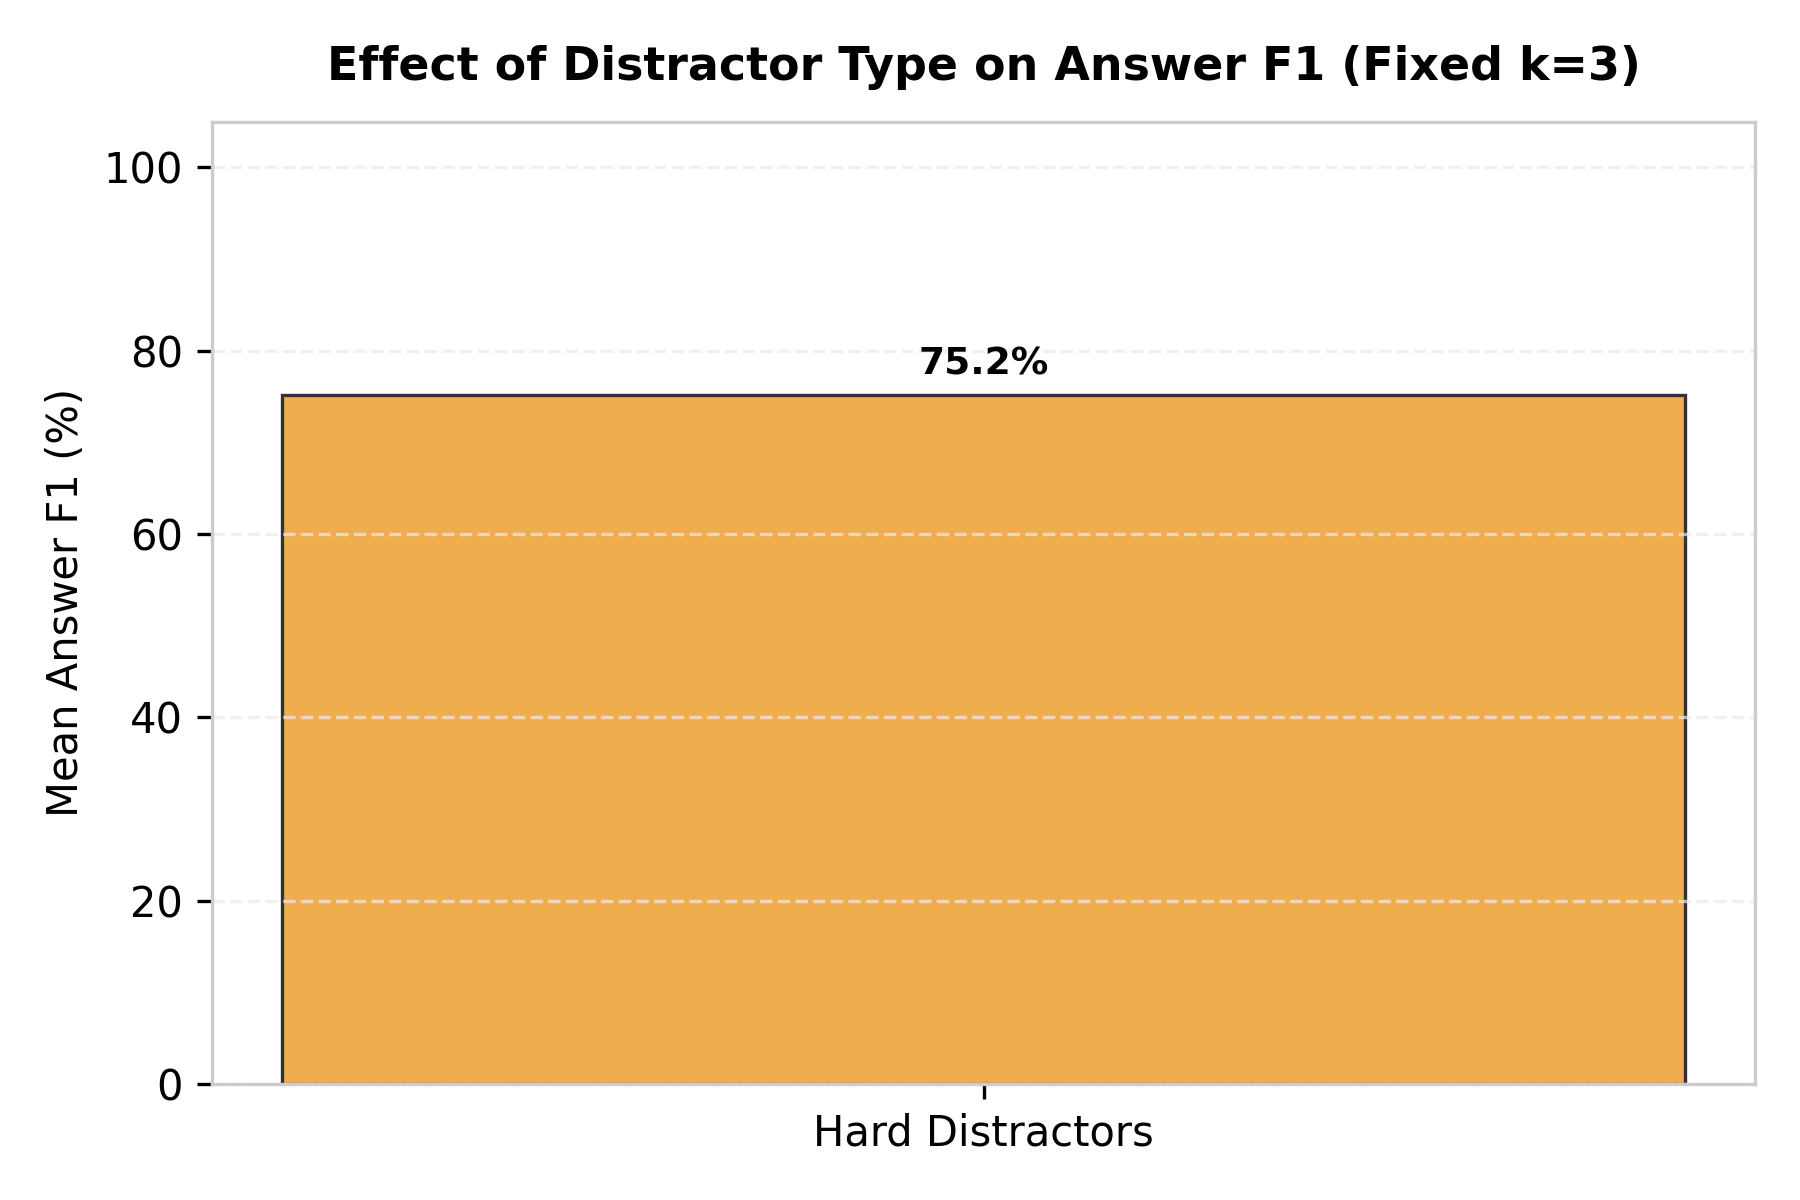
\includegraphics[width=0.85\columnwidth]{figures/distractor_type_comparison.png}
\caption{Comparison of Answer F1 between Random and Hard Distractors at fixed $k=3$ (Experiment B).}
\label{fig:distractor_types}
\end{figure}

Figure~\ref{fig:distractor_types} highlights the impact of distractor semantic hardness. At identical context depth ($k=3$), hard distractors mined via BM25 induce significantly greater degradation than random corpus passages, corroborating Hypothesis 3 and the findings of \cite{sure2026}.

Furthermore, evaluating Condition D (Top-$k$ filtering) indicates that passing only the top-3 reranked documents yields competitive or superior performance compared to passing the full unranked candidate pool, confirming that context pruning reduces distracting surface interference.

\section{Failure Analysis}
Using our automated failure classifier, we identified four primary failure categories:
\begin{enumerate}
    \item \textbf{Clean Correct to Noisy Incorrect}: Passages containing overlapping entities diluted reader attention, causing the model to extract incorrect dates or neighboring proper nouns.
    \item \textbf{Reranker False Positives}: Occurrences where a hard distractor scored higher than the gold passage due to excessive keyword matching, displacing gold evidence down the context window.
    \item \textbf{Reranking Recovery}: Cases where placing the gold passage into position 0 completely restored correct answer extraction from an otherwise failing candidate set.
\end{enumerate}

\section{Discussion}
Our findings confirm that context noise is not benign in RAG architectures. Reader models exhibit significant distractibility even in single-gold setups. Importantly, cross-encoder rerankers provide a high-leverage mitigation without requiring retraining the generation model, solely by optimizing evidence ordering.

\section{Limitations and Threats to Validity}
\begin{itemize}
    \item \textbf{Single-Gold Scope}: Experiments inject exactly one supportive gold passage alongside distractors. Multi-hop synthesis across multiple supportive passages was not evaluated.
    \item \textbf{Domain Specificity}: Evaluations were conducted on Wikipedia-derived SQuAD 1.1; conversational or clinical domains may exhibit different noise dynamics.
    \item \textbf{Model Capacity}: While compact models clearly demonstrate noise sensitivity, larger frontier models (e.g., 70B+) possess higher attention capacity and may exhibit different saturation plateaus.
\end{itemize}

\section{Conclusion}
RobustRAG establishes an open, reproducible undergraduate research framework for evaluating context noise in Retrieval-Augmented Generation. Our controlled experiments reveal that distractor quantity and lexical hardness severely impair question answering, while cross-encoder reranking serves as an effective, computationally accessible mitigation. The entire framework, datasets, and Streamlit dashboard are open-source and run locally on standard hardware.

\bibliographystyle{IEEEtran}
\bibliography{references}

\end{document}
